\documentclass{article}
\usepackage{amsmath}
\usepackage{tikz}
\usepackage{graphicx}

\begin{document}

\begin{center}
    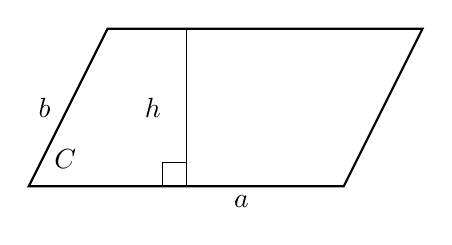
\begin{tikzpicture}
        % Draw the parallelogram
        \draw[thick] (0,0) -- (4,0) -- (5,2) -- (1,2) -- cycle;
        
        % Draw solid height line
        \draw[] (2,0) -- (2,2);
        
        % Draw right angle symbol
        \draw (2,0) -- (2,0.3) -- (1.7,0.3) -- (1.7,0) -- cycle;  % right angle symbol
        
        % Labels
        \node at (2.7,0) [below] {$a$};  % Base a
        \node at (0,1) [right] {$b$};  % Height h
        \node at (1.8,1) [left] {$h$};  % Side b
        \node at (0.2,.1) [above right] {$C$};  % Angle C
    \end{tikzpicture}

    \hspace{2cm}  % Spacing between diagram and equations

    \begin{minipage}{3cm}
        \[
        A = ah
        \]
        \[
        A = ab \sin C
        \]
    \end{minipage}

    \vspace{1cm}

    \textbf{Parallelogram}
\end{center}

\end{document}
